% Generated by `python -m experiments.experiment_2.appendix_captions` -- do not edit by hand.
% Appendix figures for Experiment 2. Needs \usepackage{graphicx,subcaption}; paths are relative to outputs/finals/experiment-2/.

\begin{figure}[p]
  \centering
  \begin{subfigure}{\textwidth}\centering
    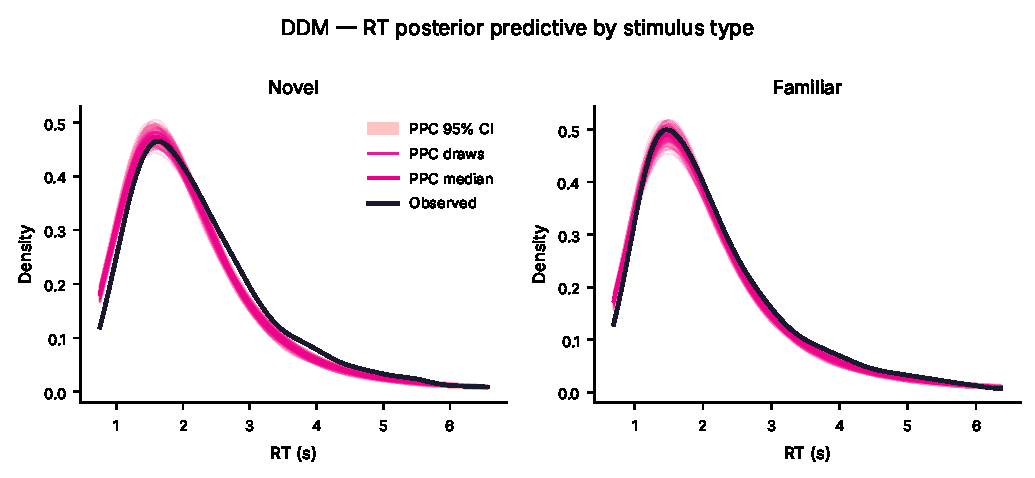
\includegraphics[width=\textwidth]{ddm/rt_ppc_stim_type.pdf}
    \caption{}
  \end{subfigure}\\[1ex]
  \begin{subfigure}{\textwidth}\centering
    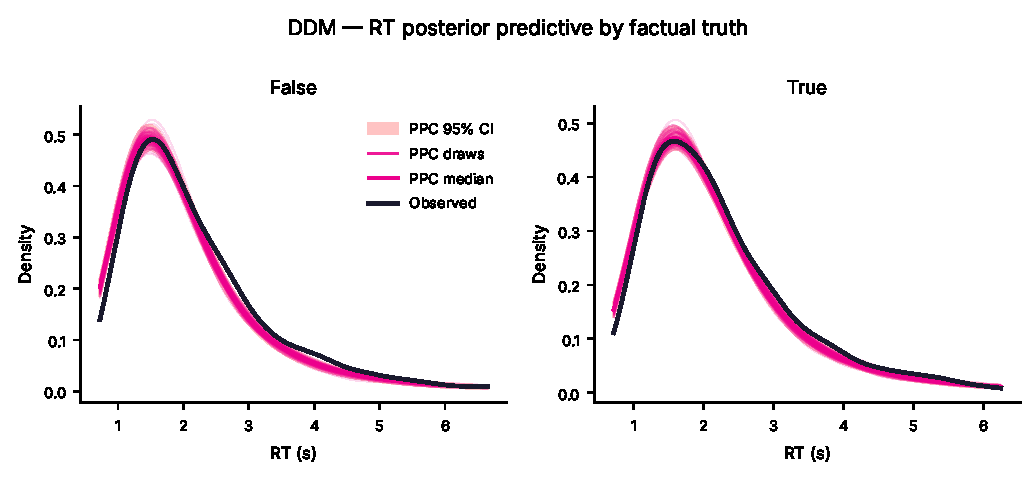
\includegraphics[width=\textwidth]{ddm/rt_ppc_truth.pdf}
    \caption{}
  \end{subfigure}
  \caption{\textbf{RT distributions, DDM: posterior predictive check.} Pooled over the 72 subjects, by (a) stimulus type and (b) factual truth: the observed RT density (black) against the posterior predictive of CogFormer's fit, one predictive data set per posterior draw (500 draws, each simulating every subject's own trials and design, then pooled), shown as a subset of individual draws (thin lines), their median (dark line) and the central 95\% band. Densities are Gaussian kernel density estimates (Silverman bandwidth), plotted between the 1st and 99th percentiles of the observed RTs. All subsequent figures in this section (Figures~\ref{fig:app2-rdm-rt}--\ref{fig:app2-cdm-angle}) follow this layout and encoding.}
  \label{fig:app2-ddm-rt}
\end{figure}

\begin{figure}[p]
  \centering
  \begin{subfigure}{\textwidth}\centering
    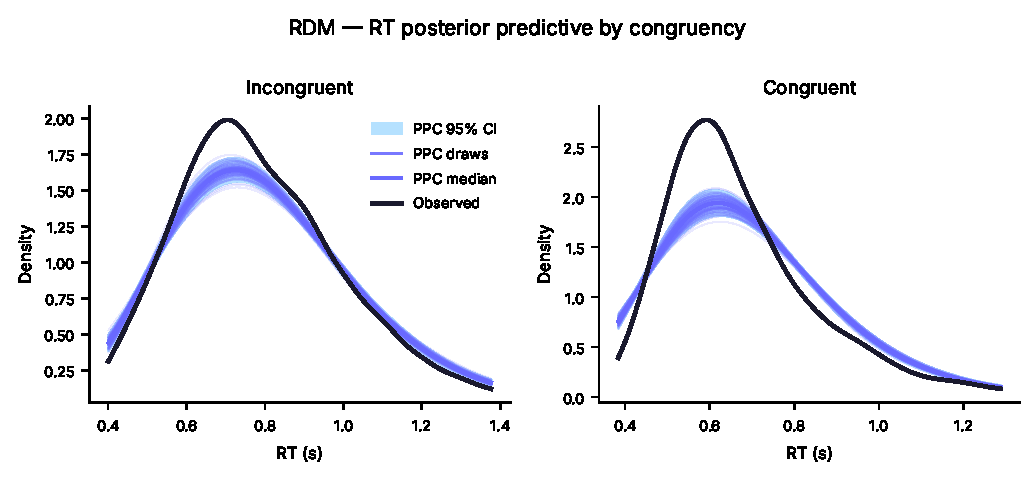
\includegraphics[width=\textwidth]{rdm/rt_ppc_congruency.pdf}
    \caption{}
  \end{subfigure}\\[1ex]
  \begin{subfigure}{\textwidth}\centering
    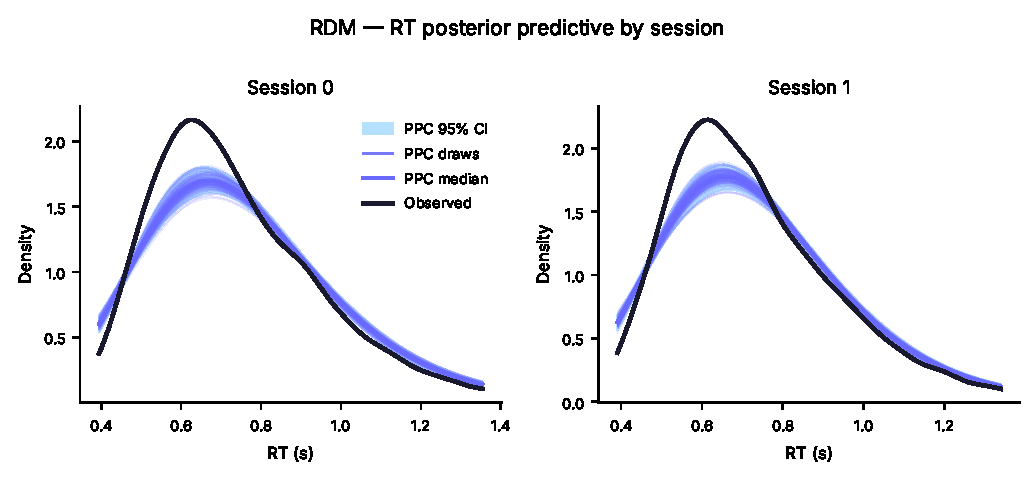
\includegraphics[width=\textwidth]{rdm/rt_ppc_session.pdf}
    \caption{}
  \end{subfigure}
  \caption{\textbf{RT distributions, RDM: posterior predictive check.} Pooled over the 149 subjects, by (a) congruency and (b) session. Encoding as in Figure~\ref{fig:app2-ddm-rt}.}
  \label{fig:app2-rdm-rt}
\end{figure}

\begin{figure}[p]
  \centering
  \begin{subfigure}{\textwidth}\centering
    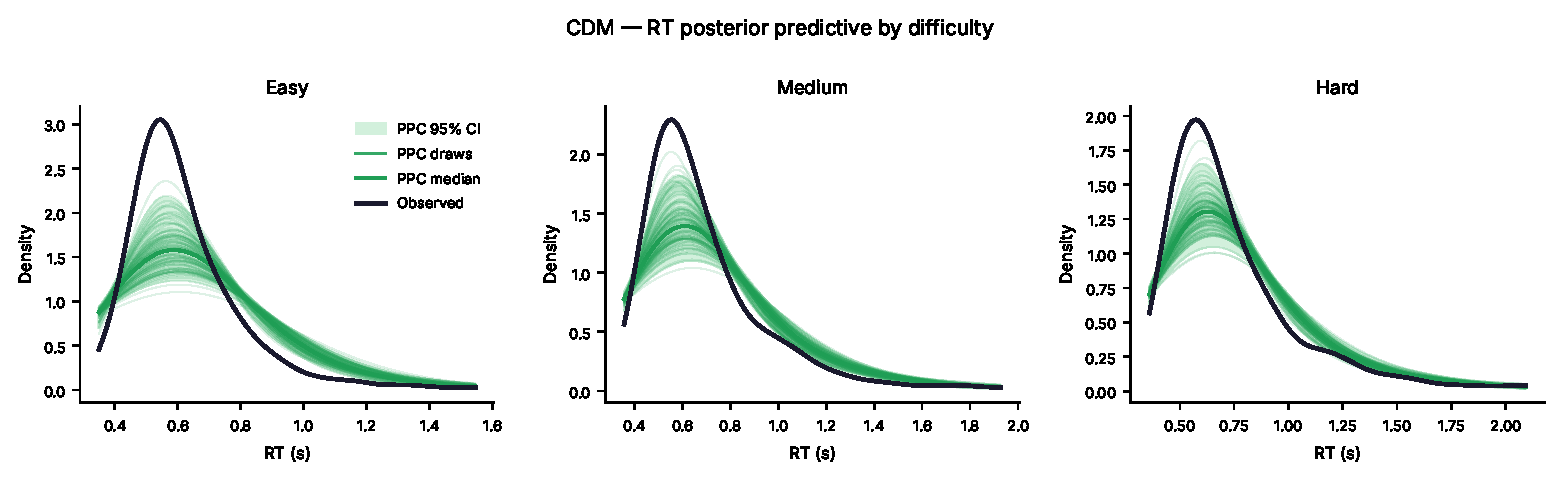
\includegraphics[width=\textwidth]{cdm/rt_ppc_difficulty.pdf}
    \caption{}
  \end{subfigure}\\[1ex]
  \begin{subfigure}{\textwidth}\centering
    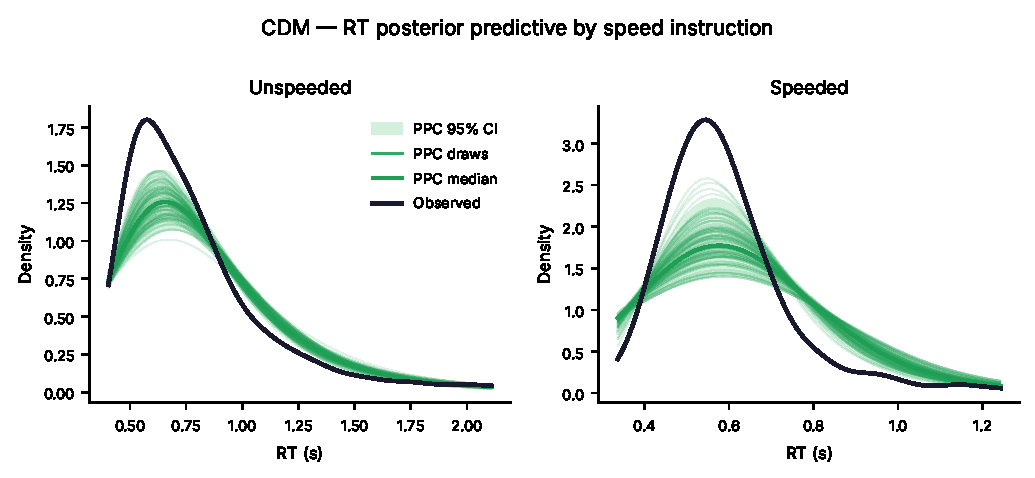
\includegraphics[width=\textwidth]{cdm/rt_ppc_speed.pdf}
    \caption{}
  \end{subfigure}
  \caption{\textbf{RT distributions, CDM: posterior predictive check.} Pooled over the 12 subjects, by (a) difficulty and (b) speed instruction. Encoding as in Figure~\ref{fig:app2-ddm-rt}.}
  \label{fig:app2-cdm-rt}
\end{figure}

\begin{figure}[p]
  \centering
  \begin{subfigure}{\textwidth}\centering
    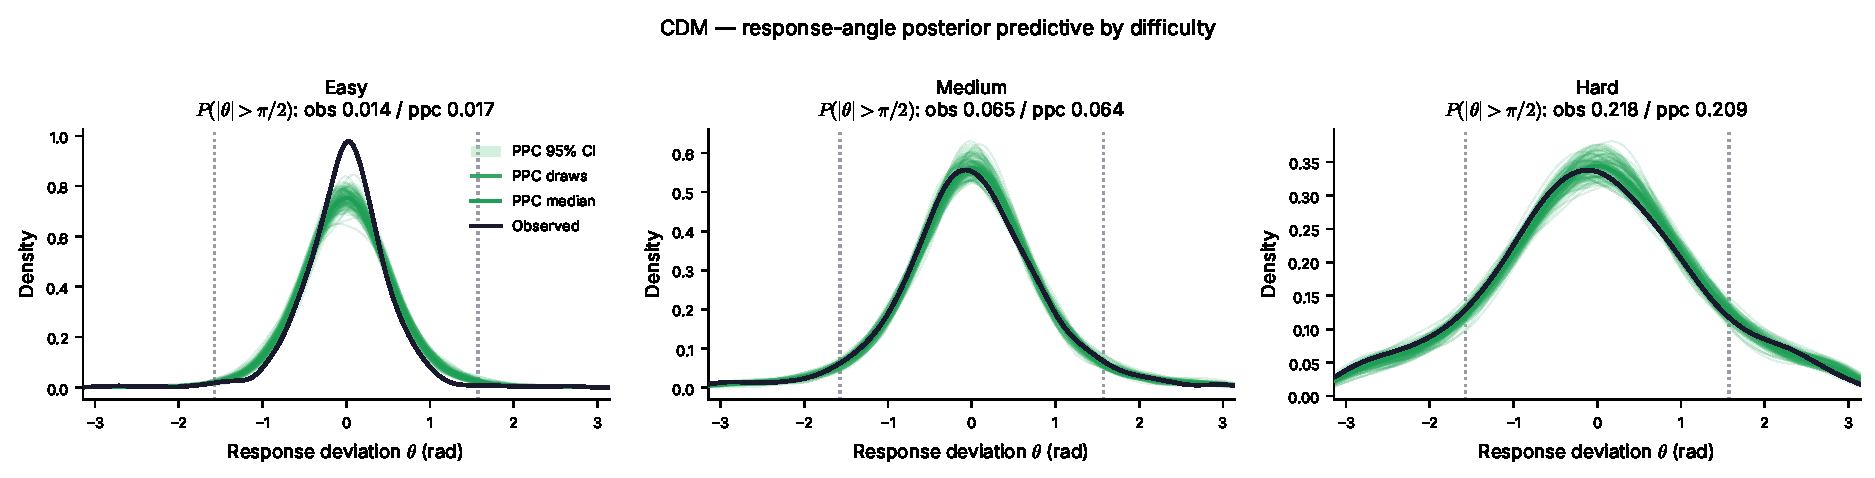
\includegraphics[width=\textwidth]{cdm/choice_ppc_difficulty.pdf}
    \caption{}
  \end{subfigure}\\[1ex]
  \begin{subfigure}{\textwidth}\centering
    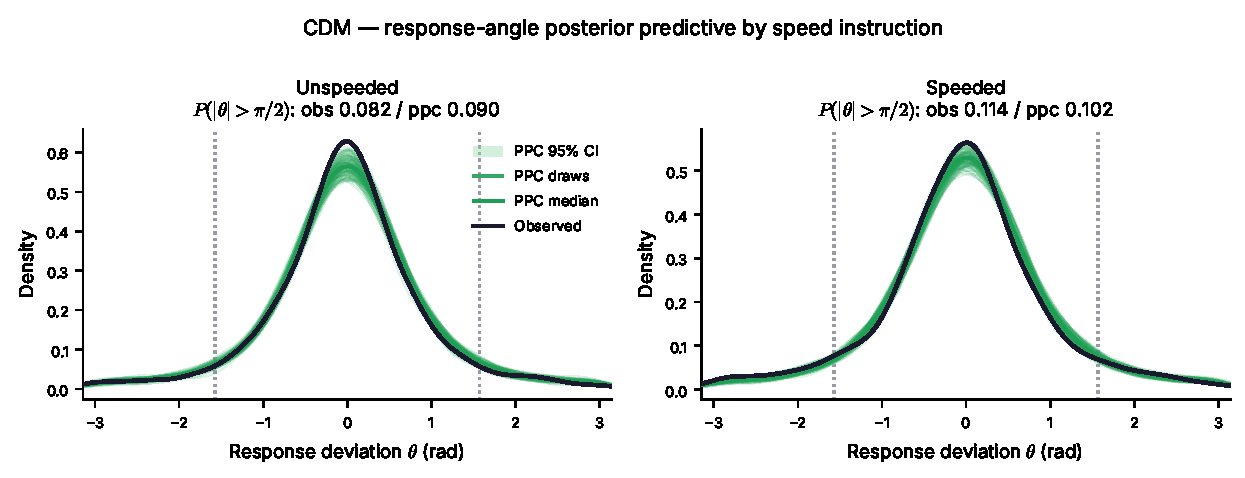
\includegraphics[width=\textwidth]{cdm/choice_ppc_speed.pdf}
    \caption{}
  \end{subfigure}
  \caption{\textbf{Response-angle distributions, CDM: posterior predictive check.} Pooled over the 12 subjects, by (a) difficulty and (b) speed instruction: the density of the response deviation $\theta$ (radians, on the model's $[-\pi, \pi]$ scale), encoded as in Figure~\ref{fig:app2-ddm-rt}. Dotted lines mark $\theta = \pm\pi/2$; each panel reports the observed and predictive share of responses beyond them, $P(|\theta| > \pi/2)$.}
  \label{fig:app2-cdm-angle}
\end{figure}
